\documentclass[tikz,border=20pt]{standalone}
\usepackage{amsmath}
\usetikzlibrary{positioning, arrows.meta, fit, backgrounds}

\begin{document}
	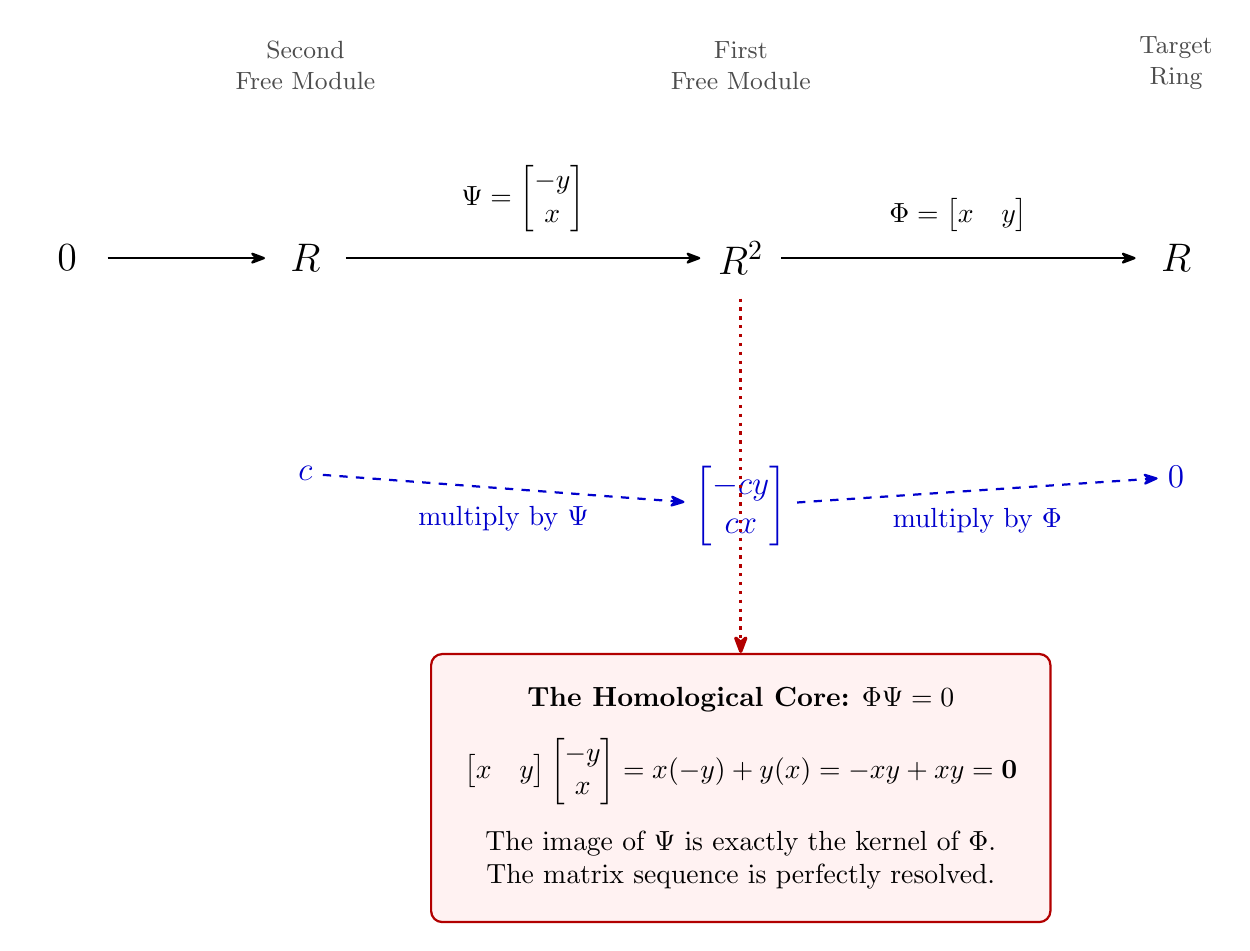
\begin{tikzpicture}[
		>={Stealth[round]}, thick,
		module/.style={font=\Large\bfseries, minimum size=1cm},
		map/.style={->, font=\normalsize},
		element/.style={font=\large},
		note/.style={font=\small\color{black!70}, align=center}
		]
		
		% --- 1. The Exact Sequence of Modules ---
		\node[module] (0L) {$0$};
		\node[module, right=2cm of 0L] (R1) {$R$};
		\node[module, right=4.5cm of R1] (R2) {$R^2$};
		\node[module, right=4.5cm of R2] (R3) {$R$};
		
		\draw[map] (0L) -- (R1);
		\draw[map] (R1) -- node[above=0.2cm] {$\Psi = \begin{bmatrix} -y \\ x \end{bmatrix}$} (R2);
		\draw[map] (R2) -- node[above=0.2cm] {$\Phi = \begin{bmatrix} x & y \end{bmatrix}$} (R3);
		
		% Annotations for the modules
		\node[note, above=1.5cm of R1] {Second\\Free Module};
		\node[note, above=1.5cm of R2] {First\\Free Module};
		\node[note, above=1.5cm of R3] {Target\\Ring};
		
		% --- 2. The Element Flow ---
		\node[element, text=blue!80!black, below=2cm of R1] (e1) {$c$};
		\node[element, text=blue!80!black, below=2cm of R2] (e2) {$\begin{bmatrix} -cy \\ cx \end{bmatrix}$};
		\node[element, text=blue!80!black, below=2cm of R3] (e3) {$0$};
		
		\draw[|->, map, blue!80!black, dashed] (e1) -- node[below=0.1cm] {multiply by $\Psi$} (e2);
		\draw[|->, map, blue!80!black, dashed] (e2) -- node[below=0.1cm] {multiply by $\Phi$} (e3);
		
		% --- 3. The Composition Proof Box ---
		\node[draw=red!70!black, fill=red!5, rounded corners, align=center, inner sep=12pt, below=4.5cm of R2] (proof) {
			\textbf{The Homological Core:} $\Phi \Psi = 0$ \\[0.3cm]
			$\begin{bmatrix} x & y \end{bmatrix} \begin{bmatrix} -y \\ x \end{bmatrix} = x(-y) + y(x) = -xy + xy = \mathbf{0}$ \\[0.3cm]
			\normalsize The image of $\Psi$ is exactly the kernel of $\Phi$. \\
			\normalsize The matrix sequence is perfectly resolved.
		};
		
		% Connecting arrows to the proof box
		\draw[->, red!70!black, dotted, very thick] (R2) -- (proof);
		
	\end{tikzpicture}
\end{document}